%1218
\newpage
\subsection{絵を\ruby{重}{かさ}ねて表示してみよう}


もう少し別な絵を表示してみましょう。

スクリプトエディタの、ファイル→「開く」メニューから「apple.hsp」を読み込んで実行してみてください。

\begin{figure}[H]
    \begin{center}
      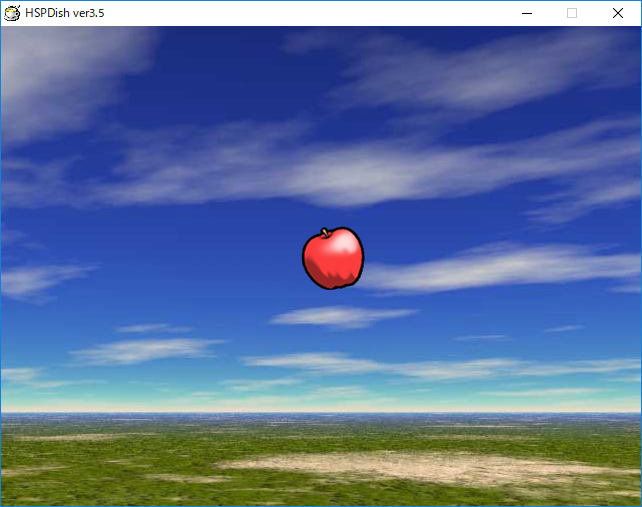
\includegraphics[keepaspectratio,width=9.634cm,height=7.599cm]{text04-img/s_applehsp.png}
      \caption{apple.hspの実行画面}
    \end{center}
    \label{fig:prog_menu}
\end{figure}

今度は、画面の中央に「りんご」が表示されていることに気付いたでしょうか。


実は、このプログラムでは背景と「りんご」の2つの画像を使っています。

背景の上に「りんご」を表示しているのです。


\begin{figure}[H]
    \begin{center}
      
\includegraphics[keepaspectratio,width=2.249cm,height=2.249cm]{text04-img/text04-img016.png}
      \caption{リンゴの画像( apple.png )}
    \end{center}
    \label{fig:prog_menu}
\end{figure}


\begin{figure}[H]
    \begin{center}
      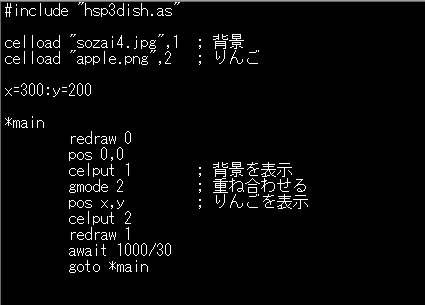
\includegraphics[keepaspectratio,width=11.245cm,height=8.07cm]{text04-img/text04-img017.png}
    \end{center}
    \label{fig:prog_menu}
\end{figure}

このように複数の番号を登録して、celput命令を使うことで絵を重ねて表示することができます。

そのために、gmodeという新しい命令が使われています。


\begin{description}
    \item \textgt{\bf \ \ (HSPのルール)}
\end{description}


\begin{description}
    \item \textgt{\bf \ \ 画像を重ねる設定をするにはgmode命令を使います}
    \item \textgt{\bf \ \ gmodeの後、スペースに続けてコピーモードを示す数字を指定します}
    \item \textgt{\bf \ \ コピーモードは、以下のような意味があります}
    \item \textgt{\bf \ \ \ \ 0のとき \ \ \ \ \ \ \ : 画像のまま表示}
    \item \textgt{\bf \ \ \ \ 1か2のとき \ \ \ : 透明な部分は背景を残して表示}
    \item \textgt{\bf \ \ \ \ 3のとき \ \ \ \ \ \ \ : 透明度を変えて表示}
\end{description}

「gmode 2」を指定することで、リンゴの透明な部分は背景が表示されて、きれいに重なっているように見えています。試しに、「gmode 0」にしてリンゴの絵がどのように表示されるか確認してみましょう。

リンゴのように透明な部分がある絵は、以前にも使ったGIMPツールで作ったり、確認することができます。GIMPは、画像ファイルの右クリックメニューから「GNU Image Manipulation Program」を選択することで起動させることができます。

\begin{figure}[H]
    \begin{center}
      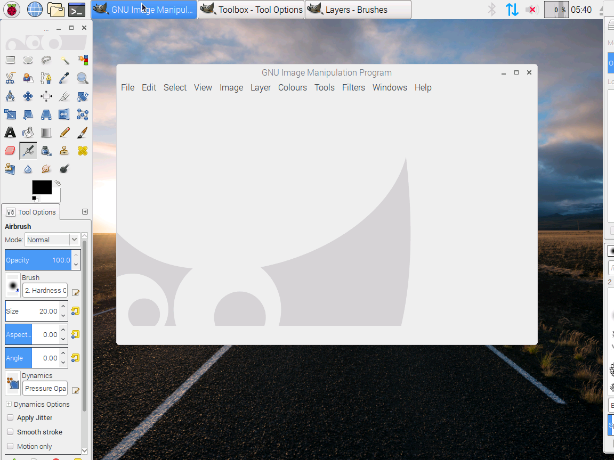
\includegraphics[keepaspectratio,width=7.091cm,height=5.318cm]{text04-img/text04-img018.png}
      \caption{GIMPを起動した画面}
    \end{center}
    \label{fig:prog_menu}
\end{figure}

celput命令には、実はもっと多くのパラメーターがあります。



\begin{description}
    \item \textgt{\bf \ \ celput 絵の番号, \ruby{分割画像}{ぶん|かつ|が|ぞう}No. , \ruby{横方向}{よこ|ほう|こう}の\ruby{表示倍率}{ひょう|じ|ばい|りつ}, \ruby{縦方向}{たて|ほう|こう}の\ruby{表示倍率}{ひょう|じ|ばい|りつ}, \ruby{回転角度}{かい|てん|かく|ど}}
\end{description}



\begin{description}
    \item \textgt{\bf \ \ 横方向の表示倍率=0.0〜    : 横方向の表示倍率(\ruby{実数}{じっ|すう})}
    \item \textgt{\bf \ \ 縦方向の表示倍率=0.0〜    : 縦方向の表示倍率(\ruby{実数}{じっ|すう})}
    \item \textgt{\bf \ \ 回転角度=0.0〜6.28…(2π) : 回転角度(\ruby{実数}{じっ|すう})}
\end{description}

絵を自由な大きさ(\ruby{倍率}{ばい|りつ})、\ruby{角度}{かく|ど}で出すことができるようになっています。

通常は、倍率1、角度0の状態で表示されます。

分割画像No.は、1つの画像を複数の小さなブロックに分けて表示するための機能です。

(これについては、また別の機会に説明します。)

試しに、表示倍率や角度を変えてみて、どのように表示が変わるか確認してみましょう。

また、余裕がある人は、文字を重ねてさらに複雑な画面を作ることに挑戦してください。


%1372






